\documentclass{beamer}

% Copyright 2010 Drow Ltd.
% 
% In principle, this file can be redistributed and/or modified under
% the terms of the GNU Public License, version 2.
% 
% However, this file is supposed to be a template to be modified
% for your own needs. For this reason, if you use this file as a
% template and not specifically distribute it as part of a another
% package/program, I grant the extra permission to freely copy and
% modify this file as you see fit and even to delete this copyright
% notice. 
\mode<presentation>
{
  \usetheme[titleline=true,
  alternativetitlepage=true,
  titlepagelogo=images/Java_logo]{Torino}
  \usecolortheme{nouvelle}
  \beamertemplatenavigationsymbolsempty
}

\usepackage{times}
\usepackage[utf8]{inputenc}
\usepackage[english,bulgarian]{babel}
\usepackage[T2A]{fontenc}

\usepackage{listings}
\lstset{language=Java,
  captionpos=b,
  tabsize=4,
  keywordstyle=\color{blue},
  commentstyle=\color{gray},
  stringstyle=\color{green},
  numbers=left,
  breaklines=true,
  showstringspaces=false,
  basicstyle=\ttfamily,
  emph={label},
  frame=shadowbox, 
  rulesepcolor=\color{blue},
  columns=fixed}

\title{Наследяване и полиморфизъм}

\author{инж. Божидар ~Бацов}

\institute{Drow Ltd.}

\date{16.11.2010}

\subject{Talks}
% This is only inserted into the PDF information catalog. Can be left
% out. 

\begin{document}

\begin{frame}
  \titlepage
\end{frame}

\begin{frame}{Съдържание}
  \transdissolve
  \tableofcontents[pausesections]
\end{frame}

\section{Наследяване}

\subsection{Модификатори за достъп}
\begin{frame}{Модификатори за достъп}
  \transdissolve
  \begin{itemize}
    \item Ограничават видимостта на класовете и техните членове \pause
    \item Могат да се прилагат върху класове, методи и полета \pause
    \begin{itemize}
    \item \textcolor{blue}{private}
      \begin{itemize}
      \item достъп само в рамките на класа
      \end{itemize} \pause
    \item \textcolor{blue}{public}
      \begin{itemize}
      \item достъп за всички
      \end{itemize} \pause
    \item default(package)
      \begin{itemize}
      \item достъп за всички в пакета
      \end{itemize} \pause
    \item \textcolor{blue}{protected}
      \begin{itemize}
      \item default + достъп в наследените
      \end{itemize} \pause
    \end{itemize}    
  \end{itemize}
\end{frame}

\subsection{Основни концепции}
\begin{frame}{Наследяване}
  \transdissolve
  \begin{itemize}
  \item Фундаментална техника в ООП \pause
  \item Изграждане на нови класове върху основата на съществуващи
    класове \pause
  \item Преизползват се методите и полетата на съществуващи класове \pause
  \item Добавя се ново поведение и състояние \pause
  \item Променя се съществуващото поведение
  \end{itemize}
\end{frame}

\begin{frame}{Концептуален пример}
  \transdissolve
  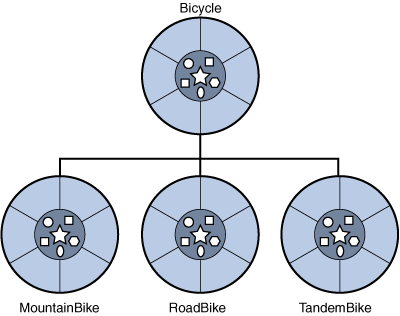
\includegraphics[width=320px, height=150px]{images/concepts-inheritance.png}  
\end{frame}

\begin{frame}{От общото към частното}
  \transdissolve
  \begin{itemize}
  \item наследяване == разширяване \pause
  \item суперклас(клас родител/базов клас) \pause
  \item подклас(клас наследник) \pause
  \item отношението между подклас и суперклас е е(is-a)
    \begin{itemize}
      \item Планинското колело е колело.
      \item Програмистът е човек.
    \end{itemize}
  \end{itemize}
\end{frame}

\begin{frame}[fragile]
  \frametitle{Наследяване - супер клас}
  \transdissolve
\begin{lstlisting}
public class Bicycle {
    // the Bicycle class has three fields
    public int cadence;
    public int gear;
    public int speed;
    // the Bicycle class has one constructor
    public Bicycle(int startCadence, int startSpeed, int startGear) {
        gear = startGear;
        cadence = startCadence;
        speed = startSpeed;
    }
    // the Bicycle class has four methods
    public void setCadence(int newValue) {
        cadence = newValue;
    }
    public void setGear(int newValue) {
        gear = newValue;
    }
    public void applyBrake(int decrement) {
        speed -= decrement;
    }
    public void speedUp(int increment) {
        speed += increment;
    }
}
\end{lstlisting}
\end{frame}

\begin{frame}[fragile]
  \frametitle{Наследяване - подклас}
  \transdissolve
\begin{lstlisting}
public class MountainBike extends Bicycle {
	
    // the MountainBike subclass adds one field
    public int seatHeight;

    // the MountainBike subclass has one constructor
    public MountainBike(int startHeight, int startCadence, int startSpeed, int startGear) {
        super(startCadence, startSpeed, startGear);
        seatHeight = startHeight;
    }	
	
    // the MountainBike subclass adds one method
    public void setHeight(int newValue) {
        seatHeight = newValue;
    }	

}
\end{lstlisting}
\end{frame}

\subsection{Ключови моменти}
\begin{frame}{Ключови моменти при наследяването}
  \transdissolve
  \begin{itemize}
  \item Подкласът наследява всички \textcolor{blue}{public} и
    \textcolor{blue}{protected} членове на суперкласа, независимо от
    пакетите в които се намират \pause
  \item Подкласът наследява и членовете с достъп default, ако са
    намира в същия пакет като суперкласа \pause
  \item Конструкторът на подкласа извиква конструктора на суперкласа \pause
  \item \textcolor{blue}{private} елементите не са достъпни директно в
    подкласовете \pause
  \item Ключовата дума \textcolor{blue}{super} позволява обръщение към метод от
    суперкласа
  \end{itemize}
\end{frame}

\begin{frame}{Какво можете да правите в подклас?}
  \transdissolve
  \begin{itemize}
  \item Може да използвате наследените полета както обикновените
    полета \pause
  \item Може да декларирате поле в подклас със същото име, като такова
    в суперклас и по този начин ще го скриете(лош стил) \pause
  \item Може да декларирате нови полета в подкласа \pause
  \item Наследените методи могат да се използват директно \pause
  \item Може да създавате instance методи в подклас със същата
    сигнатура, като методи от суперкласа и по този начин ще ги
    предефинирате(override) \pause
  \item Същото нещо при статични методи ще доведе то скриването им \pause
  \item Може да дефинирате нови методи \pause
  \item Може(Винаги) конструктор в подкласа да извиква конструктор от
    суперкласа
  \end{itemize}
\end{frame}

\subsection{Йерархия на наследяването}
\begin{frame}{Йерархия на наследяването}
  \transdissolve
  \begin{itemize}
  \item Единична йерархия на наследяване - един подклас може да има
    само един суперклас \pause
  \item Избягват се много от проблемите на C++ \pause
  \item Интерфейсите предлагат подобие на множествено наследяване
  \end{itemize}
\end{frame}

\begin{frame}{Множествено наследяване}
  \transdissolve
  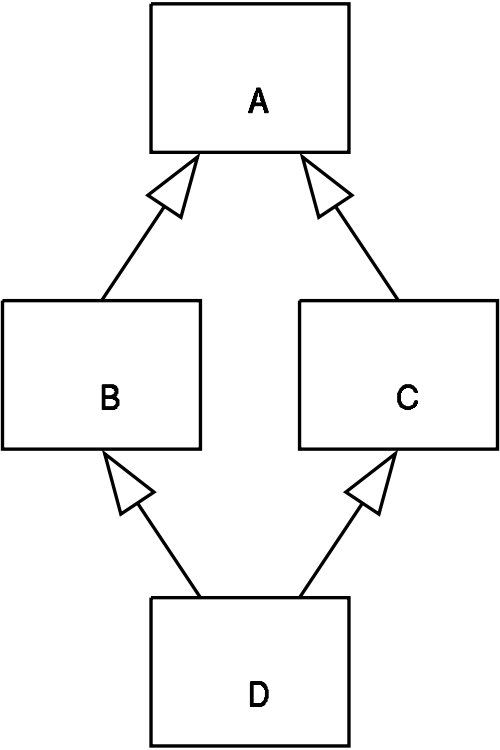
\includegraphics[width=320px, height=150px]{images/diamond_inheritance.png}
\end{frame}

\section{Полиморфизъм}

\subsection{Концепция и предимства}
\begin{frame}[fragile]
  \frametitle{Полиморфизъм}
  \transdissolve
  \begin{itemize}
    \item Променливи от суперклас могат да бъдат асоциирани с обекти
      от подкласове \pause
    \item Виртуалната машина знае истинските типове на обектите и по
      време на изпълнение извиква техните методи, независимо с
      променлива от какъв тип са асоциирани \pause
    \item Полиморфизмът е тясно свързан с късното свързване на
    методите(late binding). \pause
  \end{itemize}
  \begin{lstlisting}
Programmer p = new Programmer();
Employee e = new Programmer();
  \end{lstlisting}
\end{frame}

\begin{frame}{Предимства на полиморфизма}
  \transdissolve
  \begin{itemize}
  \item Ниска свързаност(loose coupling) \pause
  \item Гъвкавост
    \begin{itemize}
    \item нови класове могат да бъдат добавяни през
      прекомпилиране на кода
    \end{itemize}
  \item Простота
    \begin{itemize}
    \item придържаме ме се към по-прост интерфейс
    \end{itemize}
  \end{itemize}
\end{frame}

\begin{frame}{Търсене на метод}
  \transdissolve
  \begin{itemize}
  \item Търсене от компилатора(ранно/статично свързване) \pause
  \item Търсене от виртуалната машина(късно/динамично свързване) \pause
  \item Таблица на методите
  \end{itemize}
\end{frame}

\begin{frame}{Късно свързване}
  \transdissolve
  \begin{itemize}
  \item Виртуалната машина знае истинския тип на всеки един обект \pause
  \item Виртуалната машина изпълнява методите на базата на истинския
    тип \pause
  \item Необходимост за реализиране на полиморфизъм
  \end{itemize}
\end{frame}

\begin{frame}{Забраняване на наследяването и късното свързване}
  \transdissolve
  \begin{itemize}
  \item final class - неразширяем клас \pause
  \item final method - метод, който не може да бъде динамично свързан \pause
  \item Във final class всички методи са имплицитно final \pause
  \item final като оптимизационна и защитна техника
  \end{itemize}
\end{frame}

\subsection{Абстрактни класове}
\begin{frame}{Абстрактни класове}
  \transdissolve
  \begin{itemize}
  \item Създадени да бъдат разширявани \pause
  \item Не могат да бъдат инстанцирани \pause
  \item Обикновено са на върха на йерархията на наследяването \pause
  \item Съдържат един или повече методи без имплементация(абстрактни методи)
  \end{itemize}
\end{frame}

\begin{frame}[fragile]
  \frametitle{Абстрактни класове - пример}
  \transdissolve
\begin{lstlisting}
abstract class SomeClass {
    abstract void doSomething();
}

SomeClass sc = new SomeClass(); // ERROR
\end{lstlisting}
\end{frame}

\begin{frame}[fragile]
  \frametitle{Преобразуване на обекти}
  \transdissolve
  \begin{itemize}
  \item Всеки обект от подклас и е обект от суперкласа \pause
  \item Обратното не е вярно \pause
  \end{itemize}
\begin{lstlisting}
Programmer p = new Programmer();
Employee e = p;

e = new Employee();
p = e; //ERROR
\end{lstlisting}
\end{frame}

\begin{frame}[fragile]
  \frametitle{Преобразуване на обекти}
  \transdissolve
  \begin{itemize}
  \item Референция от суперклас може да бъде конвертирана до
    референция от подклас изрично
    \begin{lstlisting}
Employee e = new Programmer();
Programmer p = (Programmer) e;
    \end{lstlisting}
  \item Изричното преобразуване е опасна операция, която може да
    доведе го грешки по време на изпълнение на програмата
  \end{itemize}
\end{frame}

\begin{frame}[fragile]
  \frametitle{Преобразуване на обекти}
  \transdissolve
  \begin{itemize}
  \item Сигурно преобразуване с instanceof
    \begin{lstlisting}
if (e instanceof Programmer) {
  p = (Programmer) e;
}
    \end{lstlisting}
  \item Невъзможните преобразувания се улавят от компилатора
    \begin{lstlisting}
Date d = (Date) e;
    \end{lstlisting}
  \end{itemize}
\end{frame}

\begin{frame}{Върховния суперклас Object}
  \transdissolve
  \begin{itemize}
  \item Начало на класовата йерархия в Java \pause
  \item Всеки клас имплицитно наследява Object \pause
  \item Съдържа в себе си методи, които имат смисъл за всички обекти
    \begin{itemize}
      \item clone()
      \item equals()
      \item hashCode()
      \item toString()
    \end{itemize}
  \item Всяка референция може да бъде преобразувана до тип Object \pause
  \end{itemize}
\end{frame}

\begin{frame}{Върховния суперклас Object}
  \transdissolve
  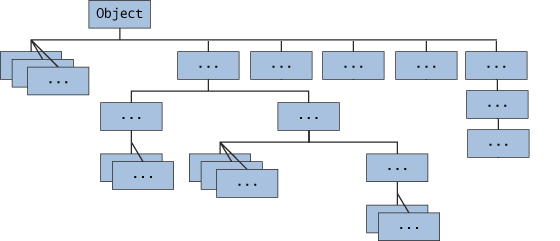
\includegraphics[width=320px, height=150px]{images/classes-object.png}
\end{frame}

\begin{frame}{Сравняване на обекти}
  \transdissolve
  \begin{itemize}
  \item == сравнява референции - сравнение за идентичност \pause
  \item метода equals() \pause
  \item Дефиниране на подходящ метод equals() \pause
    \begin{itemize}
      \item проверка за сравнение с null \pause
      \item проверка за сравнение със същия обект \pause
      \item проверка за сравнение с различен тип \pause
      \item сравняване на двата обекта по полета \pause
      \begin{itemize}
        \item рекурсивно сравняване на полета от референтни типове с equals
      \end{itemize}
    \end{itemize}
  \item връзка между equals и hashCode \pause
  \end{itemize}
\end{frame}

\begin{frame}{Модификатор за достъп protected}
  \transdissolve
  \begin{itemize}
  \item Еквивалент на default достъп + директен достъп в подкласовете \pause
  \item Употребата му се счита за лош стил \pause
  \item protected и default е желателно да бъдат избягвани \pause
  \item четири нива на достъп
    \begin{itemize}
      \item private
      \item public
      \item default(package)
      \item protected
    \end{itemize}
  \item три модификатора за достъп \pause
    \begin{itemize}
      \item private
      \item public
      \item protected
    \end{itemize}
  \end{itemize}
\end{frame}

\begin{frame}{Упражнение}
  \transdissolve
  Моделирайте йерархия от геометрични обекти:
  \begin{itemize}
    \item Circle
    \item Rectangle
    \item Square
  \end{itemize}
  За всички от тях трябва да имаме възможност да пресмятаме обиколката и
  площта ми. Използвайте абстрактен базов клас като корен на тази
  йерархия от класове.
\end{frame}

\section*{Заключение}

\begin{frame}{Заключение}
  \transdissolve
  % Keep the summary *very short*.
  \begin{itemize}
  \item
    Наследяването \alert{е мощна техника за преизползване на код и
      моделиране на отношенията между различни типове}.
  \item
    То НЕ е единствената такава техника - композицията често е за предпочитане.
  \item
    Модификаторите за достъп контролират какво точно се случва при наследяване.
  \end{itemize}
  
  % The following outlook is optional.
  \vskip0pt plus.5fill
  \begin{itemize}
  \item
    Следващият път:
    \begin{itemize}
    \item
      Интерфейси
    \item
      Вътрешни класове
    \end{itemize}
  \end{itemize}
\end{frame}

\begin{frame}{Въпроси}
  \transdissolve
  \begin{center}
    \LARGEТук е момента да зададете вашите въпроси! :-)
  \end{center}
\end{frame}

\begin{frame}{Край}
  \transdissolve
  \begin{center}
    \LARGEБлагодаря Ви за вниманието!
  \end{center}
\end{frame}

\end{document}

%%% Local Variables: 
%%% mode: latex
%%% TeX-master: t
%%% End: 
